\documentclass[12pt]{iopart}

% --- PACKAGES ---
\usepackage{iopams}     % IOP math symbols
\usepackage{graphicx}   % Graphics support
\usepackage[colorlinks=true, linkcolor=blue, citecolor=blue, urlcolor=blue]{hyperref}
% NOTE: iopart often works fine without 'cite'. If you see compilation issues, remove the next line.
\usepackage{cite}
% Optional: ORCID. If it causes issues on your system, remove the next line and \orcidlink in \author.
\usepackage{orcidlink}
\usepackage{placeins}

% Optional (robustness with older LaTeX setups):
% \usepackage[T1]{fontenc}
% \usepackage[utf8]{inputenc}

\begin{document}

% --- TITLE PAGE ---
\title[Discrete Relational Network Dynamics]{Discrete Relational Network Dynamics (DRND): A Fully Emergent Framework for Spacetime, Matter, and the Evolution of Fundamental Constants}

\author{Robert K\l{}eczek$^{1}$\,\orcidlink{0009-0009-9774-0446}}
\address{$^{1}$Independent Researcher}
\ead{r.kleczek@advocem.com}

\vspace{10pt}
\begin{indented}
\item[]\textbf{Version 1.0.1} -- February 2026
\end{indented}

\begin{abstract}
Contemporary cosmology exhibits persistent internal tensions, including discrepancies in late- and early-Universe inferences of the Hubble parameter and open questions surrounding the physical origin of the Dark Sector. Most extensions of the concordance model modify the stress-energy content while retaining a smooth background manifold and fixed fundamental constants.
Here we \emph{outline} Discrete Relational Network Dynamics (DRND), a background-independent framework in which spacetime, matter degrees of freedom, and effective dynamical laws emerge from an evolving discrete graph of causal relations. Dimensionality is treated as a dynamical, scale- and environment-dependent property characterized by the network's spectral dimension $d_S$ defined via diffusion on the graph.
Within a minimal toy description based on random-walk transport, we \emph{propose} that the effective signal-propagation speed $c_{\mathrm{eff}}$ can depend on the network topology, with high-connectivity phases (large $d_S$) enabling faster causal processing and low-connectivity/percolative regimes (reduced $d_S$) inducing longer traversal times. We discuss a phenomenological parameterization in which $c_{\mathrm{eff}}(z)$ modifies cosmological distance measures and can mimic part of the phenomenology usually attributed to Dark Energy under the assumption of constant $c$. We also formulate a qualitative screening picture in which virialized regions remain effectively three-dimensional ($d_S \simeq 3$), suppressing local detectability.
The paper is intended as a framework and a set of falsifiable directions, and we explicitly separate heuristic scaling relations from future work required for full dynamical consistency and data fitting (SNe, BAO, CMB).
\end{abstract}

\vspace{2pc}
\noindent{\it Keywords}: Emergent Spacetime, Quantum Gravity, VSL Theory, Dark Energy, Spectral Dimension, Network Theory

\maketitle

% --- MAIN CONTENT ---

\section{Introduction: The Case for Full Emergence}

The $\Lambda$CDM model remains an exceptionally successful effective description, yet several observations motivate renewed scrutiny of its foundational assumptions. In particular, the mismatch between late-Universe and early-Universe inferences of the Hubble parameter and the rapid emergence of massive structures at high redshift suggest that aspects of cosmic history may be miscalibrated within the standard pipeline \cite{Riess2022,Labbe2023}. Many proposed extensions address these issues by modifying the matter sector (additional fields, exotic fluids, interacting dark components) while preserving a smooth background manifold and fixed fundamental constants.

In this work we explore a complementary hypothesis: that the tension may be partially rooted not in the choice of stress-energy content but in the assumption that spacetime geometry and ``constants'' are fundamental inputs rather than emergent outputs. We propose a paradigm of \textbf{Full Emergence}, in which the universe is described at the most basic level by a discrete, evolving graph of causal relations. In this view, spacetime is not a pre-existing container and particles are not primitive objects within it; both arise as effective, coarse-grained descriptions of the same underlying relational substrate.

Within DRND, the core identifications are:
\begin{itemize}
    \item \textbf{Space} as an emergent property of adjacency relations in the graph.
    \item \textbf{Time} as the ordering induced by sequential updates of network states (causal dynamics).
    \item \textbf{Matter} as topologically stable, localized excitations (graph solitons/knots).
    \item \textbf{Effective constants} ($c, h, G$) as parameters of coarse-grained transport and response, determined by the network's statistical connectivity.
\end{itemize}

A central technical device is the \textbf{spectral dimension} $d_S$, defined operationally via diffusion on the graph \cite{Ambjorn2005}. Unlike integer manifold dimension, $d_S$ can vary with scale and environment, allowing dense regions and sparse void-like regions to exhibit different effective transport properties. We then examine a minimal toy parameterization in which an environment-dependent $c_{\mathrm{eff}}$ modifies cosmological distance measures. This creates a concrete pathway by which a topology-driven effect could mimic part of the observational signature commonly attributed to Dark Energy, while remaining screened in virialized regions.

We emphasize from the outset: this paper presents a framework and heuristic scaling relations meant to sharpen falsifiable predictions. A fully dynamical treatment (including consistency with conservation laws, background evolution, and joint fits to SNe/BAO/CMB) is deferred to subsequent work.

\subsection{Scope and limitations}
DRND is introduced here as (i) an explicit ontology (an evolving relational graph), (ii) operational definitions of effective dimension and transport (diffusion/random walks), and (iii) a phenomenological parameterization of environment- and redshift-dependent propagation. In this version we do \emph{not} claim a complete derivation of cosmological background dynamics, nor a full statistical fit to data. Statements labeled as ``heuristic'' should be read as ans\"atze motivated by network transport theory and intended to guide near-term falsification.

Key open requirements for a complete theory include explicit graph update rules and coarse-graining maps to continuum observables, dynamical consistency with conservation identities in the presence of variable effective parameters, and joint constraints from SNe, BAO, CMB, BBN, and local precision tests.

\section{The Ontology of the Network}

We define the universe as a directed graph $G(V, E)$ consisting of a vertex set $V$ and a directed edge set $E$.
DRND adopts an \textbf{event ontology}:
\begin{enumerate}
    \item A \textbf{node} $v \in V$ is not a spatial point, but an \textit{elementary causal event} (a fundamental unit of interaction or ``becoming'').
    \item An \textbf{edge} $(v_i, v_j) \in E$ represents a direct causal influence: event $v_i$ is an immediate precursor to $v_j$.
\end{enumerate}
In this view, the graph does not exist \textit{in} spacetime; rather, spacetime emerges from the graph. A fundamental microscopic length scale can be associated with the discreteness (often taken to be of order the Planck length $L_P$), while logical time corresponds to sequential growth or update of the event set.

We abandon the assumption of a fixed integer dimensionality. Instead, the effective dimension of space is defined by the \textbf{spectral dimension} $d_S$, determined by diffusion processes on the graph structure \cite{Ambjorn2005}. Operationally, if $P_r(\tau)$ denotes the return probability of a random walker after $\tau$ steps (graph-time), then
\begin{equation}
P_r(\tau) \sim \tau^{-d_S/2}.
\end{equation}
Consequently, dimensionality becomes a dynamical, environment-dependent observable. Dense, highly clustered regions can exhibit $d_S \gtrsim 3$, while sparse, tree-like regions (voids) may exhibit $d_S < 3$.

\section{Minimal Toy Model: Measuring \texorpdfstring{$d_S$}{dS} and Defining \texorpdfstring{$c_{\mathrm{eff}}$}{ceff} on Graphs}
\label{sec:toy}

This section introduces a minimal operational layer used throughout the paper: how $d_S$ and an effective propagation speed can be defined directly on a graph. The purpose is not to fix a unique microscopic dynamics, but to specify measurable quantities whose scaling can be falsified in toy simulations and, ultimately, mapped to cosmological observables.

\subsection{Random-walk operator and return probability}
Let $A$ be the adjacency matrix of the (possibly directed) graph and $k_i$ the out-degree of node $i$. For a simple (unbiased) random walk on a directed graph one may define a transition matrix
\begin{equation}
P_{ij} = \frac{A_{ij}}{k_i},
\end{equation}
assuming $k_i>0$ for relevant nodes. The $\tau$-step transition probability is $(P^\tau)_{ij}$. The return probability averaged over nodes is
\begin{equation}
P_r(\tau) = \left\langle (P^\tau)_{ii} \right\rangle_i.
\end{equation}
An effective (scale-dependent) spectral dimension can be extracted from the slope
\begin{equation}
d_S(\tau) = -2\,\frac{d\ln P_r(\tau)}{d\ln \tau}.
\end{equation}
In practice $d_S(\tau)$ may flow with $\tau$, capturing scale dependence, and can vary between environments.

\subsection{Mean first-passage time and an effective propagation speed}
To define an effective signal speed, one needs (i) a notion of distance on the graph and (ii) a notion of traversal time. A natural distance is the directed (or symmetrized) shortest-path length $d_G(i,j)$ (graph geodesic). A natural traversal time for diffusive/transport processes is the mean first-passage time (MFPT) $T_{FP}(i\to j)$ for a random walker starting at $i$ to first reach $j$.

We define an environment- and scale-dependent effective propagation speed by averaging over node pairs within a region $\mathcal{R}$:
\begin{equation}
c_{\mathrm{eff}}(\mathcal{R}) \;\equiv\;
\frac{\left\langle d_G(i,j)\right\rangle_{i,j\in\mathcal{R}}}{\left\langle T_{FP}(i\to j)\right\rangle_{i,j\in\mathcal{R}}}\, \ell_0,
\end{equation}
where $\ell_0$ is a microscopic length per edge used to set units (e.g. $\ell_0 \sim L_P$). In highly connected ``small-world'' graphs, $\langle d_G\rangle$ decreases and MFPT tends to decrease; in sparse/percolative regimes, $\langle d_G\rangle$ and MFPT can increase due to tortuosity/backbone constraints. This provides a concrete mechanism by which topology can influence effective signal propagation.

\subsection{Ansatz linking \texorpdfstring{$c_{\mathrm{eff}}$}{ceff} to \texorpdfstring{$d_S$}{dS}}
The above definitions allow one to test whether a monotonic relationship exists between $d_S$ and $c_{\mathrm{eff}}$ in families of graphs. Motivated by the expectation that higher connectivity (larger $d_S$) enables faster coarse-grained transport, we use the phenomenological ansatz
\begin{equation}
c_{\mathrm{eff}}(d_S) = c_0 \left(\frac{d_S}{3}\right)^\gamma,
\label{eq:cds}
\end{equation}
with $\gamma>0$ a coupling parameter. Equation (\ref{eq:cds}) is not claimed as a theorem; it is a compact parameterization to be confronted with toy simulations and, if viable, with observational constraints after mapping to cosmological propagation effects.

\subsection{Operational procedure (toy graphs)}
For a given graph ensemble, the following operational steps define $d_S(\tau)$ and $c_{\mathrm{eff}}$:
\begin{enumerate}
\item \textbf{Generate a graph instance} $G$ with $N$ nodes (e.g. small-world or percolation cluster).
\item \textbf{Define the random-walk transition matrix} $P_{ij}=A_{ij}/k_i$.
\item \textbf{Estimate return probability} $P_r(\tau)$ and extract $d_S(\tau)$.
\item \textbf{Compute MFPT} and geodesic distance to obtain $c_{\mathrm{eff}}$.
\item \textbf{Correlate} $c_{\mathrm{eff}}$ with $\bar d_S$ across graph instances.
\end{enumerate}

\begin{figure}[htbp]
\centering
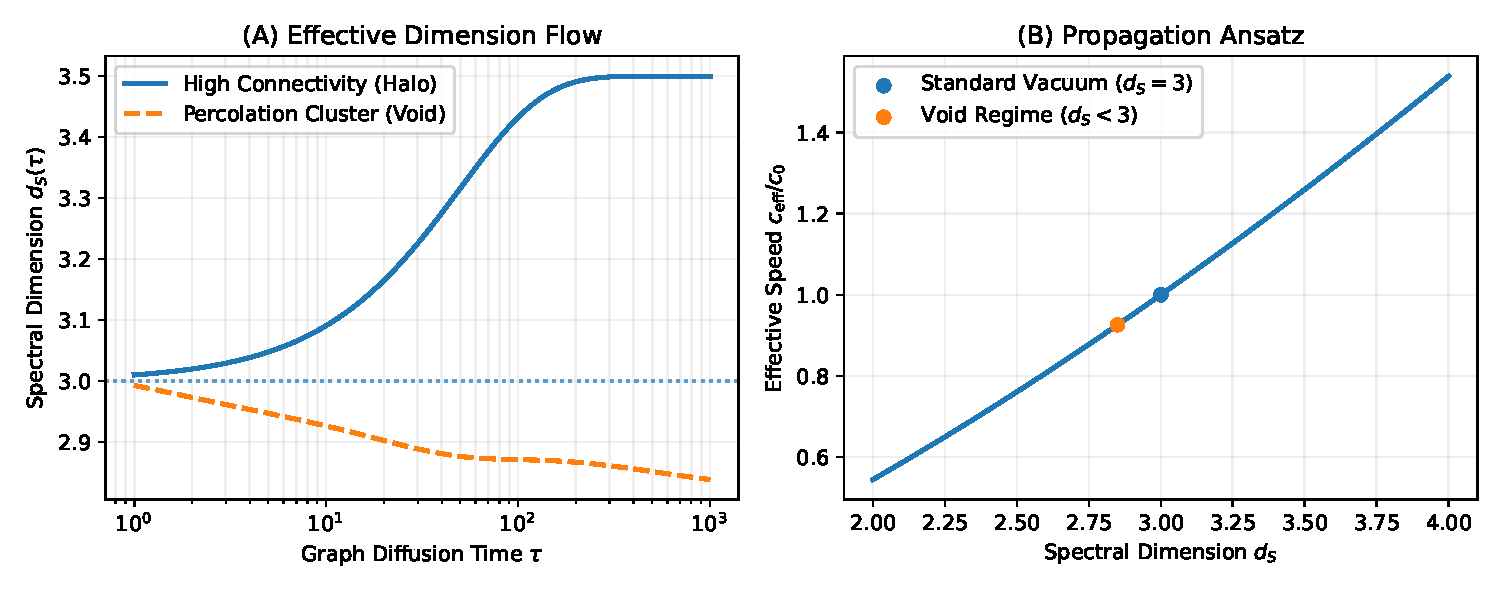
\includegraphics[width=0.95\textwidth]{figures/toy_drnd_ds_ceff.pdf}
\caption{Toy-network diagnostics for DRND. \textbf{(A)} Scale-dependent spectral dimension $d_S(\tau)$ estimated from random-walk return probability on representative small-world and percolative graph instances. \textbf{(B)} Correlation of effective propagation speed $c_{\mathrm{eff}}$ (defined via mean first-passage times) with an averaged spectral dimension $\bar d_S$ across graph ensembles. The plot illustrates the monotonicity motivating the phenomenological parameterization $c_{\mathrm{eff}}(d_S)=c_0(d_S/3)^\gamma$.}
\label{fig:toy_ds_ceff}
\end{figure}

\section{Covariant Evolution of Effective Constants}

The central novelty of DRND is that effective physical parameters can depend on the topological state of the network. In this version we treat such dependencies phenomenologically and separate them from a full derivation from graph dynamics.

\subsection{Heuristic motivation via random walks}
To motivate a possible scaling of an effective propagation speed $c_{\mathrm{eff}}$, we consider transport on fractal-like structures. The mean squared displacement scales as $\langle r^2(\tau)\rangle \sim \tau^{2/d_w}$. In percolative regimes typical of sparse, void-like connectivity, edge removal forces traversal along a tortuous backbone, increasing effective traversal times and thereby reducing $c_{\mathrm{eff}}$. This motivates the monotonic ansatz (\ref{eq:cds}).

The qualitative implications are:
\begin{itemize}
    \item \textbf{Early Universe (large $d_S$):} A hyper-connected phase can permit $c_{\mathrm{eff}} \gg c_0$, potentially alleviating the Horizon Problem \cite{Magueijo2003}.
    \item \textbf{Cosmic Voids (reduced $d_S$):} Percolative connectivity can increase tortuosity and traversal times, lowering $c_{\mathrm{eff}}$ relative to screened regions.
\end{itemize}

\subsection{On covariant scaling of \texorpdfstring{$\hbar$}{hbar} and \texorpdfstring{$G$}{G}}
Rather than asserting a unique scaling, we introduce \emph{parameter families} meant to be tested:
\begin{equation}
\hbar(t) \propto c_{\mathrm{eff}}(t)^{p}, \qquad
G(t) \propto c_{\mathrm{eff}}(t)^{q},
\label{eq:pq}
\end{equation}
with exponents $(p,q)$ to be constrained.
In this version we do not claim that any particular choice (\ref{eq:pq}) is consistent with BBN/CMB/local constraints; the goal is to isolate testable signatures of topology-dependent propagation while deferring quantitative global fits.

\section{Mapping to Cosmological Observables}
\label{sec:observables}

We state a minimal phenomenological layer:
\begin{itemize}
    \item \textbf{Redshift:} standard kinematic definition is assumed at the level of observables.
    \item \textbf{Distances:} luminosity distance is treated as a functional of an effective propagation speed along the line of sight.
\end{itemize}

\subsection{Two interpretations of \texorpdfstring{$c_{\mathrm{eff}}(z)$}{ceff(z)}}
The parameterization $c_{\mathrm{eff}}(z)\approx c_0(1+z)^\epsilon$ can be interpreted as:

\begin{itemize}
\item \textbf{(I) Environment-averaged propagation:} $c_{\mathrm{eff}}(z)$ is a volume-averaged effective speed at epoch $z$. This is simple but can wash out anisotropic, line-of-sight effects.
\item \textbf{(II) Line-of-sight (LoS) weighted propagation:} propagation depends on void fraction (or a connectivity-weighted measure) along direction $\hat{\mathbf{n}}$. This predicts environment-correlated scatter in distance indicators and time delays, enabling direct null tests.
\end{itemize}

\begin{table}[htbp]
\caption{Qualitative constraint channels for phenomenological propagation parameter $\epsilon$ and the screening picture.}
\label{tab:constraints_screening}
\begin{center}
\small
\raggedright
\begin{tabular}{p{0.22\textwidth} p{0.48\textwidth} p{0.22\textwidth}}
\hline
\textbf{Channel} & \textbf{Constraint in DRND} & \textbf{Screening status} \\
\hline
Type Ia SNe & Integrated effect on $D_L(z)$ & Unscreened (void-weighted) \\
BAO & Standard ruler consistency & Mixed \\
CMB scale/damping & Early-time propagation effects (if present) & Not assessed here \\
BBN yields & Early-time interaction/expansion rates & Must be screened or tightly limited \\
Local clocks / LLR & Local parameter variability & Screened ($d_S \simeq 3$) \\
Lensing delays & LoS environment dependence & Unscreened signature \\
\hline
\end{tabular}
\end{center}
\end{table}

\FloatBarrier
\section{Resolving the Dark Sector (Toy Phenomenology)}

\subsection{Dark Energy as Dimensional Reduction}
In standard FRW cosmology, the luminosity distance can be expressed in terms of the dimensionless expansion rate $E(z)\equiv H(z)/H_0$ and the comoving distance. In DRND we introduce a toy propagation factor $c_{\mathrm{eff}}(z)\approx c_0(1+z)^\epsilon$, which modifies the radial distance integral:
\begin{equation}
\chi(z)=\frac{c_0}{H_0}\int_0^z \frac{(1+z')^\epsilon}{E(z')}\,dz'.
\end{equation}
For $\Omega_\Lambda=0$, spatial curvature is implied with $\Omega_k=1-\Omega_m$, and
\begin{equation}
E(z)=\sqrt{\Omega_m(1+z)^3+\Omega_k(1+z)^2},\qquad \Omega_k=1-\Omega_m.
\end{equation}
The transverse comoving distance $D_M(z)$ is
\begin{equation}
D_M(z)=
\cases{
\frac{1}{\sqrt{\Omega_k}}\sinh\!\left(\sqrt{\Omega_k}\,\chi(z)\right) & for $\quad \Omega_k>0$\\
\chi(z) & for $\quad \Omega_k=0$\\
\frac{1}{\sqrt{|\Omega_k|}}\sin\!\left(\sqrt{|\Omega_k|}\,\chi(z)\right) & for $\quad \Omega_k<0$\\
}
\end{equation}
and the luminosity distance is
\begin{equation}
D_L^{\mathrm{DRND}}(z)=(1+z)\,D_M(z).
\end{equation}

{\raggedright
In $\Lambda$CDM, the expansion rate includes a Dark Energy contribution (often parameterized by $\Omega_\Lambda \approx 0.7$ in flat fits) to match supernova distance--redshift data.

In the DRND toy phenomenology, we set $\Omega_\Lambda=0$ at the background level and ask whether a topology-dependent $c_{\mathrm{eff}}(z)$ can mimic part of the same distance--redshift phenomenology without invoking vacuum energy.

We stress that this is a toy phenomenology aimed at isolating propagation effects in distance inference; consistency with a full cosmological dataset is deferred.
\par}

\subsection{Topological Screening (Qualitative Hypothesis)}
We propose a \textbf{topological screening hypothesis}:
\begin{equation}
d_S(r) \approx \cases{3 & \textrm{inside halos (screened)}\\ <3 & \textrm{in cosmic voids (unscreened)}\\}
\end{equation}
Thus, local physics remains effectively constant-$c$ at the level of precision tests, while cosmological signals traversing substantial void fractions experience an effective reduction in $c_{\mathrm{eff}}$.

\subsection{The CMB Cold Spot (Interpretive Direction)}
The framework suggests that photons traversing large supervoids may experience altered transport statistics in a low-$d_S$ regime, offering a potential interpretation of the CMB Cold Spot as a signature of reduced effective dimension. Quantitative modeling and dedicated confrontation with CMB data are deferred.

\section{Discussion and Falsifiable Directions}

DRND suggests several falsifiable directions:
\begin{enumerate}
    \item \textbf{Environment-dependent propagation tests:} strong-lensing time delays and inferred $H_0$ should correlate with the void fraction (or a connectivity proxy) along the line of sight under the LoS-weighted interpretation.
    \item \textbf{FRB/GRB timing:} transient signals may exhibit residual timing correlations with large-scale structure, after controlling for plasma dispersion and intrinsic lags.
    \item \textbf{Topological dark matter (speculative):} stable graph solitons (knots) as massive, weakly coupled degrees of freedom.
\end{enumerate}

\section{Conclusion}
We have presented DRND as a candidate framework of Full Emergence. The spectral dimension $d_S$ provides an operational measure of connectivity, enabling a topology-dependent effective propagation speed $c_{\mathrm{eff}}$. At the level of a toy phenomenology, variable $c_{\mathrm{eff}}(z)$ can bias distance--redshift inference and mimic parts of Dark Energy-like signatures, while topological screening can protect local physics. Future work will focus on explicit graph dynamics, mapping to continuum observables, and joint data fits to determine whether these transport mechanisms survive quantitative falsification.

\section*{Data and code availability}
The figure \ref{fig:toy_ds_ceff} is generated from a simple Python script included in the Zenodo deposit (together with the figure file). No observational data products were generated in this work.

\section*{Competing interests}
The author declares no competing interests.

\section*{References}
\begin{thebibliography}{99}
\bibitem{Riess2022} Riess A G \etal\ 2022 \textit{Astrophys.\ J.\ Lett.} \textbf{934} L7
\bibitem{Labbe2023} Labb\'e I \etal\ 2023 \textit{Nature} \textbf{616} 266
\bibitem{Ambjorn2005} Ambjorn J, Jurkiewicz J and Loll R 2005 \textit{Phys.\ Rev.\ Lett.} \textbf{95} 171301
\bibitem{Magueijo2003} Magueijo J 2003 \textit{Rep.\ Prog.\ Phys.} \textbf{66} 2025
\bibitem{Sorkin2003} Sorkin R D 2003 \textit{arXiv:gr-qc/0309009}
\bibitem{Einstein1916} Einstein A 1916 \textit{Annalen der Physik} \textbf{49} 769
\end{thebibliography}

\end{document}
